\documentclass[varwidth=true, border=2pt]{standalone}

\usepackage{pgfplots}
\usepackage{tikz}
\usepackage{helvet}
\usepackage[eulergreek]{sansmath}

\pgfplotsset{
tick label style = {font=\sansmath\sffamily},
every axis label/.append style={font=\sffamily\footnotesize},
}

\begin{document}
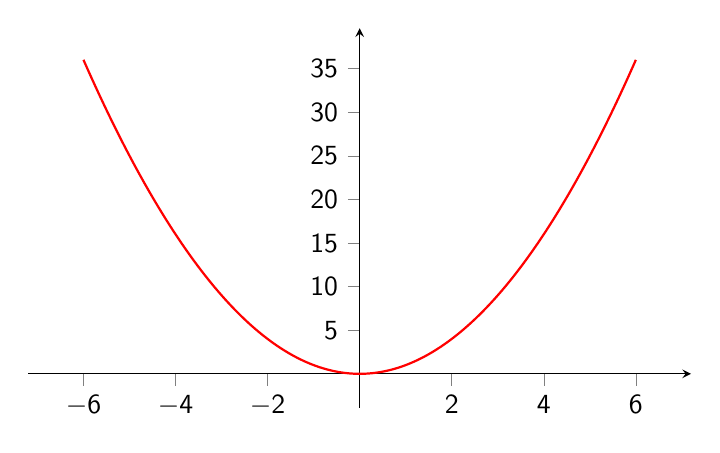
\begin{tikzpicture}
    \begin{axis}[
        % legend pos=south west,
        axis x line=middle,
        axis y line=middle,
        % grid = major,
        width=10cm,
        height=6.4cm,
        % grid style={dashed, gray!30},
        xmin=-6,     % start the diagram at this x-coordinate
        xmax= 6,     % end   the diagram at this x-coordinate
        ymin=-0.25,  % start the diagram at this y-coordinate
        ymax= 36,    % end   the diagram at this y-coordinate
        % axis background/.style={fill=white},
        xtick = {-6, -4,..., 6},
        ytick = {0, 5,..., 35},
        tick align=outside,
        enlargelimits=true,
        tension=0.08]
      \addplot[domain=-6:6, red, thick,samples=200] {x*x};
    \end{axis}
\end{tikzpicture}
\end{document}
